\documentclass[a4paper,11pt]{article}

\usepackage[dutch]{babel}
\usepackage[utf8]{inputenc}
\usepackage{a4wide,graphicx}
\usepackage{eurosym}
\usepackage{listings}
\usepackage{color}
\usepackage{hyperref}
\usepackage{comment}
\usepackage{float}
\usepackage{framed}
\usepackage{graphicx}

\lstset{numbers=left}

\begin{document}

\title{Inkapseling: Wat is het en waar is het goed voor}
\date{}

\maketitle

\section{Inkapseling in Java}

Het is in Java o.a. mogelijk te kiezen welke functies en velden van een klasse wel en welke niet voor objecten van andere klassen toegankelijk zijn.
Ook bij de eindopdracht is deze keuze van belang en we oefenen er hier in deze les alvast mee.
Het komt er op neer dat je je afvraagt wat nu eigenlijk van buitenaf bezien de essentie van iets is.
Een essentiele ``activiteit'' van een wegvoertuig is bijvoorbeeld dat 't kan rijden.
Of er een verbrandingsmotor of een electromotor in zit is van minder belang, behalve voor oliemaatschappijen.

Functies (methods) en velden van objecten die van buitenaf toegankelijk zijn, worden aangeduid met het woord \emph{public}.
Functies en velden die alleen vanuit objecten van de betreffende klasse zelf bruikbaar zijn, worden aangeduid met het woord \emph{private}.
De woorden \emph{public} en \emph{private} worden access class labels genoemd.
Er zijn er nog meer, maar die komen in latere lesseries aan de orde.

Het is nodig, bij het ontwerpen van je programma in een vroeg stadium te bedenken welke functies en velden \emph{public} moeten zijn, en welke \emph{private},
vooral als je programma groeit of anderszins verandert.
Het onderstaande verhaal, dat niet over computerprogramma's maar horloges gaat, maakt dit duidelijk.

\section{Demetrius en z'n vrouw}

\begin{framed}
Demetrius was een goudsmid die horloges maakte.
Die horloges waren beroemd over de hele wereld en hij had altijd genoeg werk.

Vaak als hij over een horloge gebogen zat, kwam z'n vrouw binnen en riep: KOFFIEEE!!
Hij schrok hier soms zo van, dat hij z'n werk uit z'n handen liet vallen,
waarna het betreffende horloge in honderden tandwieltjes, veertjes en lagertjes uitelkaar spatte.
Soms vloekte hij dan in het latijn, wat beschaafder klonk dan het was.

Op zekere dag had hij een goed idee:
Hij besloot z'n horloges op te bouwen uit een beperkt aantal modules, die op zich stabiele eenheden vormden.
Als z'n vrouw binnenkwam, kon het nu hoogstens nog gebeuren dat het horloge uiteenviel in een stuk of twintig modules.
Of de laatste module, waar hij net aan bezig was, viel uiteen in enkele tientallen tandwieltjes, maar daar viel mee te leven.

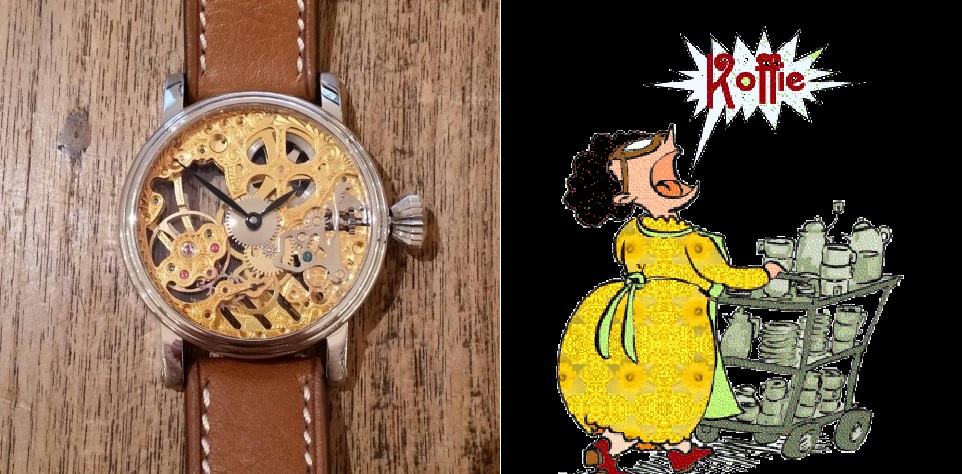
\includegraphics[width=12cm]{horloge_koffie}

Als hij er eens lekker zin in had, maakte hij een voorraadje van allerlei modules.
Wat hem echter dwars zat, is dat elke module eigenlijk maar in een soort horloge bruikbaar was.
Daarnaast ging het in elkaar schroeven van steeds maar weer de zelfde modules hem ook vervelen.

Hij schafte daarom een modulefabriekje aan, een soort robot avant la lettre.
Omdat hypes alleen ontstaan als je er wat nieuwe woorden voor verzint,
noemde hij z'n robotjes klassen, en de modules die er door werden gefabriceerd, objecten.

Wat bijzonder was aan die objecten, is dat ze zo waren ontworpen dat ze in meerder soorten horloges pasten.
Af en toe verbeterde hij z'n klassen, zodat ze efficientere objecten konden maken.
Hij zorgde er echter wel voor dat die nieuwe objecten in plaats van de oude konden worden gebruikt:
ze hadden de zelfde vorm en wijze van interactie met hun omgeving.
Omdat hij trots was op dit opnieuw briljante idee, verzon hij ook hier weer een woord voor: interface.

Hoewel zijn objecten dus een min of meer onveranderlijk interface hadden, was hij toch erg flexibel in z'n productie.
Immers kon hij de technologie binnen een object veranderen,
bijvoorbeeld van veermotor met onrustje naar kwartsgestabiliseerde synchroonmotor,
zonder dat dat enige consequenties had voor andere objecten in 't zelfde horloge,
zoals de wijzerplaat met wijzers of 't datummechanisme.

Zoals alle technici werd Demetrius er niet rijk van,
maar dat gaf niet, hij kon nu meer van z'n koffie genieten.
Zijn vondst, in de Romeinse tijd bekend als ``Divide et Impera'' (Verdeel en Heers),
heet tegenwoordig de ``Law of Demeter'' en vormt de grondslag voor Object Oriented Development.

\url{https://en.wikipedia.org/wiki/Law_of_Demeter}

Zoals je op bovenstaande webpage kunt lezen, is object orientatie geen panacee (middel tegen alle kwalen).
Het is echter wel succesvol genoeg om op ruime schaal ingang te vinden in de industrie.
Java is een typisch voorbeeld van een object georienteerde taal.
Door middel van gepast gebruik van \emph{public} en \emph{private} kun je duidelijk maken,
wat tot het interface van je objecten behoort, en wat interne details zijn, die eventueel kunnen wijzigen.
\end{framed}

\section{Objectgeorienteerde chocoladerepen}

Demetrius' werkwijze kwam in de mode en allerlei programmeertalen, van PHP tot JavaScript, kregen opeens het stempel ``object georienteerd''.
Om het kaf van het koren te scheiden werd het noodzakelijk aan te geven waaraan een object georienteerde taal moet voldoen om die naam te verdienen.
Bij een object georienteerde taal zijn minimaal de volgende conceptuele elementen aanwezig:

\begin{itemize}

\item Inkapseling: Zoals besproken, het verbergen van ontwerpbeslissingen betreffende details en het onderbrengen van deze details in een gemeenschappelijk ``omhulsel''.
Een wijd verbreid misverstand is dat het hierbij gaat om het verbergen van data.
Het gaat echter om het verbergen van datgene wat veranderlijk is.
Soms is dat de data, soms de functies die op deze data werken.
Een goed interface (public part, zie code voorbeelden) is dun (laat niet te veel zien) en stabiel (onveranderlijk).
Immers alles wat je in het interface opneemt, kun je niet zo maar meer wijzigen.
En alles wat aan het interface moet veranderen, zorgt ervoor dat ook andere objecten moeten worden aangepast.
Inkapseling vormt de hoofdmoot van wat Demetrius deed met z'n horloges.

\item Overerving: Objecten die een speciaal geval vormen van andere objecten ondersteunen minimaal hetzelfde interface.
De belangrijkste regel hier is: Do not disinherit (onterf niet).
Een versterker met een extra aansluiting voor fibre optics is OK.
Een versterker zonder cinch aansluitingen is in veel gevallen niet inpasbaar in een bestaande audio-installatie.
Doen alsof je een vogel bent, maar niet kunnen vliegen is teleurstellend, hoewel struisvogels hier anders over denken.
Maar ja, die steken hun kop in 't zand...
Naast deze ``interface inheritance'' bestaat er ook implementation inheritance.
Hierbij draait het om ``hergebruik'' van broncode.
Aanvankelijk werd dit zelfs gebracht als HET argument om object georienteerd te werken.
Echter bleek al snel dat flaws net zo inheritable waren als features.
Inkapseling (HAS A) van bestaande code bleek in veel gevallen vruchtbaarder dan overerving ervan (IS A).
Voorbeeld: De aanname dat een computer een toetsenbord en een beeldscherm BEVAT, is correcter dan de aanname dat een computer zowel een toetsenbord als een beeldscherm IS.
En correcte aannamen over de fysische objecten leiden tot betere opbouw van software objecten die hiermee moeten communiceren.

\item Veelvormigheid: Een verzameling objecten (zoals een lijst) kan heel divers zijn, zolang ze maar allemaal hetzelfde interface ondersteunen.
Dit in tegenstelling tot bijvoorbeeld een relationele database, benaderbaar in SQL.
Alle regels (records) van een tabel hebben daar hetzelfde dataformaat.
De mogelijkheid verschillende soorten objecten in dezelfde datastructuur op te nemen, opent een wereld van flexibititeit.
Omdat diverse objecten via hun overeenkomstige interface toch op een overeenkomstige manier aangesproken kunnen worden,
neemt bij gebruik van veelvormigheid de grootte van de broncode sterk af.
Immers dezelfde code kan met een verscheidenheid aan objecttypen overweg.

\end{itemize}

Alledrie deze concepten grijpen in elkaar en leiden gezamelijk tot een efficiente wijze van ontwikkelen.
Kenmerkend voor object georienteerd ontwikkelen is dat ``dingen op hun plaats vallen''.
Best practices kristalliseren uit (design patterns), de totale hoeveelheid broncode neemt af, regelmaat wordt de regel en uitzonderlingen uitzonderlijk.
Een duidelijke relatie tussen software-objecten en ``real world''-objecten is een ander kenmerk van een goed OO programma.

\section{Wat oefen je bij de twee opdrachten}

Op de slides van deze les staan twee oefenopdrachten: Het verkeerslicht en de verwarming.
Bij deze opdrachten, en bij deze lessenserie, draait het vooral om inkapseling.
Overerving en veelvormigheid komen in latere lessenseries aan de orde, maar mag je al wel gebruiken.

Let op: bij deze opdrachten gaat het niet alleen om het maken van een werkend programma.
Het is van belang dat de keuze van je interface verstandig is.
Bepaal zorgvuldig wat \emph{public} is en wat \emph{private}.
Bedenk dat wat je eenmaal in het interface stopt (\emph{public}) er niet zo maar weer uit te halen valt.
Immers andere programmeurs kunnen hun code hierop hebben gebaseerd.

Gebruik duidelijke, vanzelfsprekende namen in camel case.
Namen van klassen beginnen met een hoofdletter, alle andere namen met een kleine letter.

Vertel niet in commentaar, wat je duidelijk kunt maken in naamgeving.
Als iets \emph{temperatuur} voorstelt, noem het dan zo, en geen \emph{t}(ijd) of \emph{temp}(orary).
Bedenk dat andere ontwikkelaars ``in't echie'' mogelijk verder aan jouw software moeten werken.
Veel van wat je in deze lessenserie werkt, werpt pas z'n vruchten af bij grotere programmma's.
Software ontwerpen is vooral vooruitdenken, afwegen en structureren.
Wat je oefent is wat je leert, als je nu perfectionistisch bent, ben je straks een goede en gewilde programmeur.

\end{document}
